\documentclass[UTF8,a4paper]{article}
\usepackage{fancyhdr}
\usepackage{ctex}
\usepackage{amsmath}
\usepackage{listings}
\usepackage{color}
\usepackage{graphics}
\usepackage{graphicx}
\lstset{ %
	extendedchars=false,            % Shutdown no-ASCII compatible
	language=Matlab,                % choose the language of the code
	basicstyle=\small\sf,    % the size of the fonts that are used for the code
	tabsize=3,                            % sets default tabsize to 3 spaces
	numbers=left,                   % where to put the line-numbers
	numberstyle=\tiny,              % the size of the fonts that are used for the line-numbers
	stepnumber=1,                   % the step between two line-numbers. If it's 1 each line
	% will be numbered
	numbersep=5pt,                  % how far the line-numbers are from the code   %
	keywordstyle=\color[RGB]{33,33,234},               % keywords
	commentstyle=\color[RGB]{0,0,0},    % comments
	stringstyle=\color[rgb]{0.170,0.187,0.102},      % strings
	backgroundcolor=\color{white}, % choose the background color. You must add \usepackage{color}
	showspaces=false,               % show spaces adding particular underscores
	showstringspaces=false,         % underline spaces within strings
	showtabs=false,                 % show tabs within strings adding particular underscores                frame = single,         % adds a frame around the code
	captionpos=b,                   % sets the caption-position to bottom
	breaklines=true,                % sets automatic line breaking
	breakatwhitespace=false,        % sets if automatic breaks should only happen at whitespace
	title=\lstname,                 % show the filename of files included with \lstinputlisting;
	% also try caption instead of title
	mathescape=true,escapechar=?    % escape to latex with ?..?
	escapeinside={\%*}{*)},         % if you want to add a comment within your code
	%columns=fixed,                  % nice spacing
	%morestring=[m]',                % strings
	%morekeywords={%,...},%          % if you want to add more keywords to the set
	%    break,case,catch,continue,elseif,else,end,for,function,global,%
	%    if,otherwise,persistent,return,switch,try,while,...},%
}
\pagestyle{fancy}
\lhead{}
\chead{}
\rhead{\bfseries The Matlab Homework week 6}
\lfoot{}
\cfoot{\thepage}
\rfoot{}
\renewcommand{\headrulewidth}{0.4pt}
\begin{document}
\begin{center}
    \textbf{\LARGE{Matlab Homework week 6}}\\[0.5cm]
    \normalsize{庄震丰 22920182204393}\\[0.5cm]
    \large{Oct. $24^{th}$, 2019}
\end{center}
\section{Plot1}
\subsection{Description}
$$
    y=cosx[0.5+\frac{3sinx}{1+x^2}]
$$
divide x$\in$ [0-2$\pi$] into 101 parts,plot(x,y).
\subsection{Analysis}
Use the function plot() directly.
\subsection{Codes and Result}
\textbf{Code}
\begin{lstlisting}
    x=0:2*pi/100:2*pi;
    y=cos(x).*(0.5+3*sin(x)./(1+x.^2));
    plot(x,y);
    legend('曲线');
    title({'$y=cosx[0.5+\frac{3sinx}{1+x^2}]$'},'Interpreter','Latex');
    xlabel('x')
    ylabel('y')
\end{lstlisting}
\newpage
\textbf{Figure}
\begin{figure}[h]
    \centering
    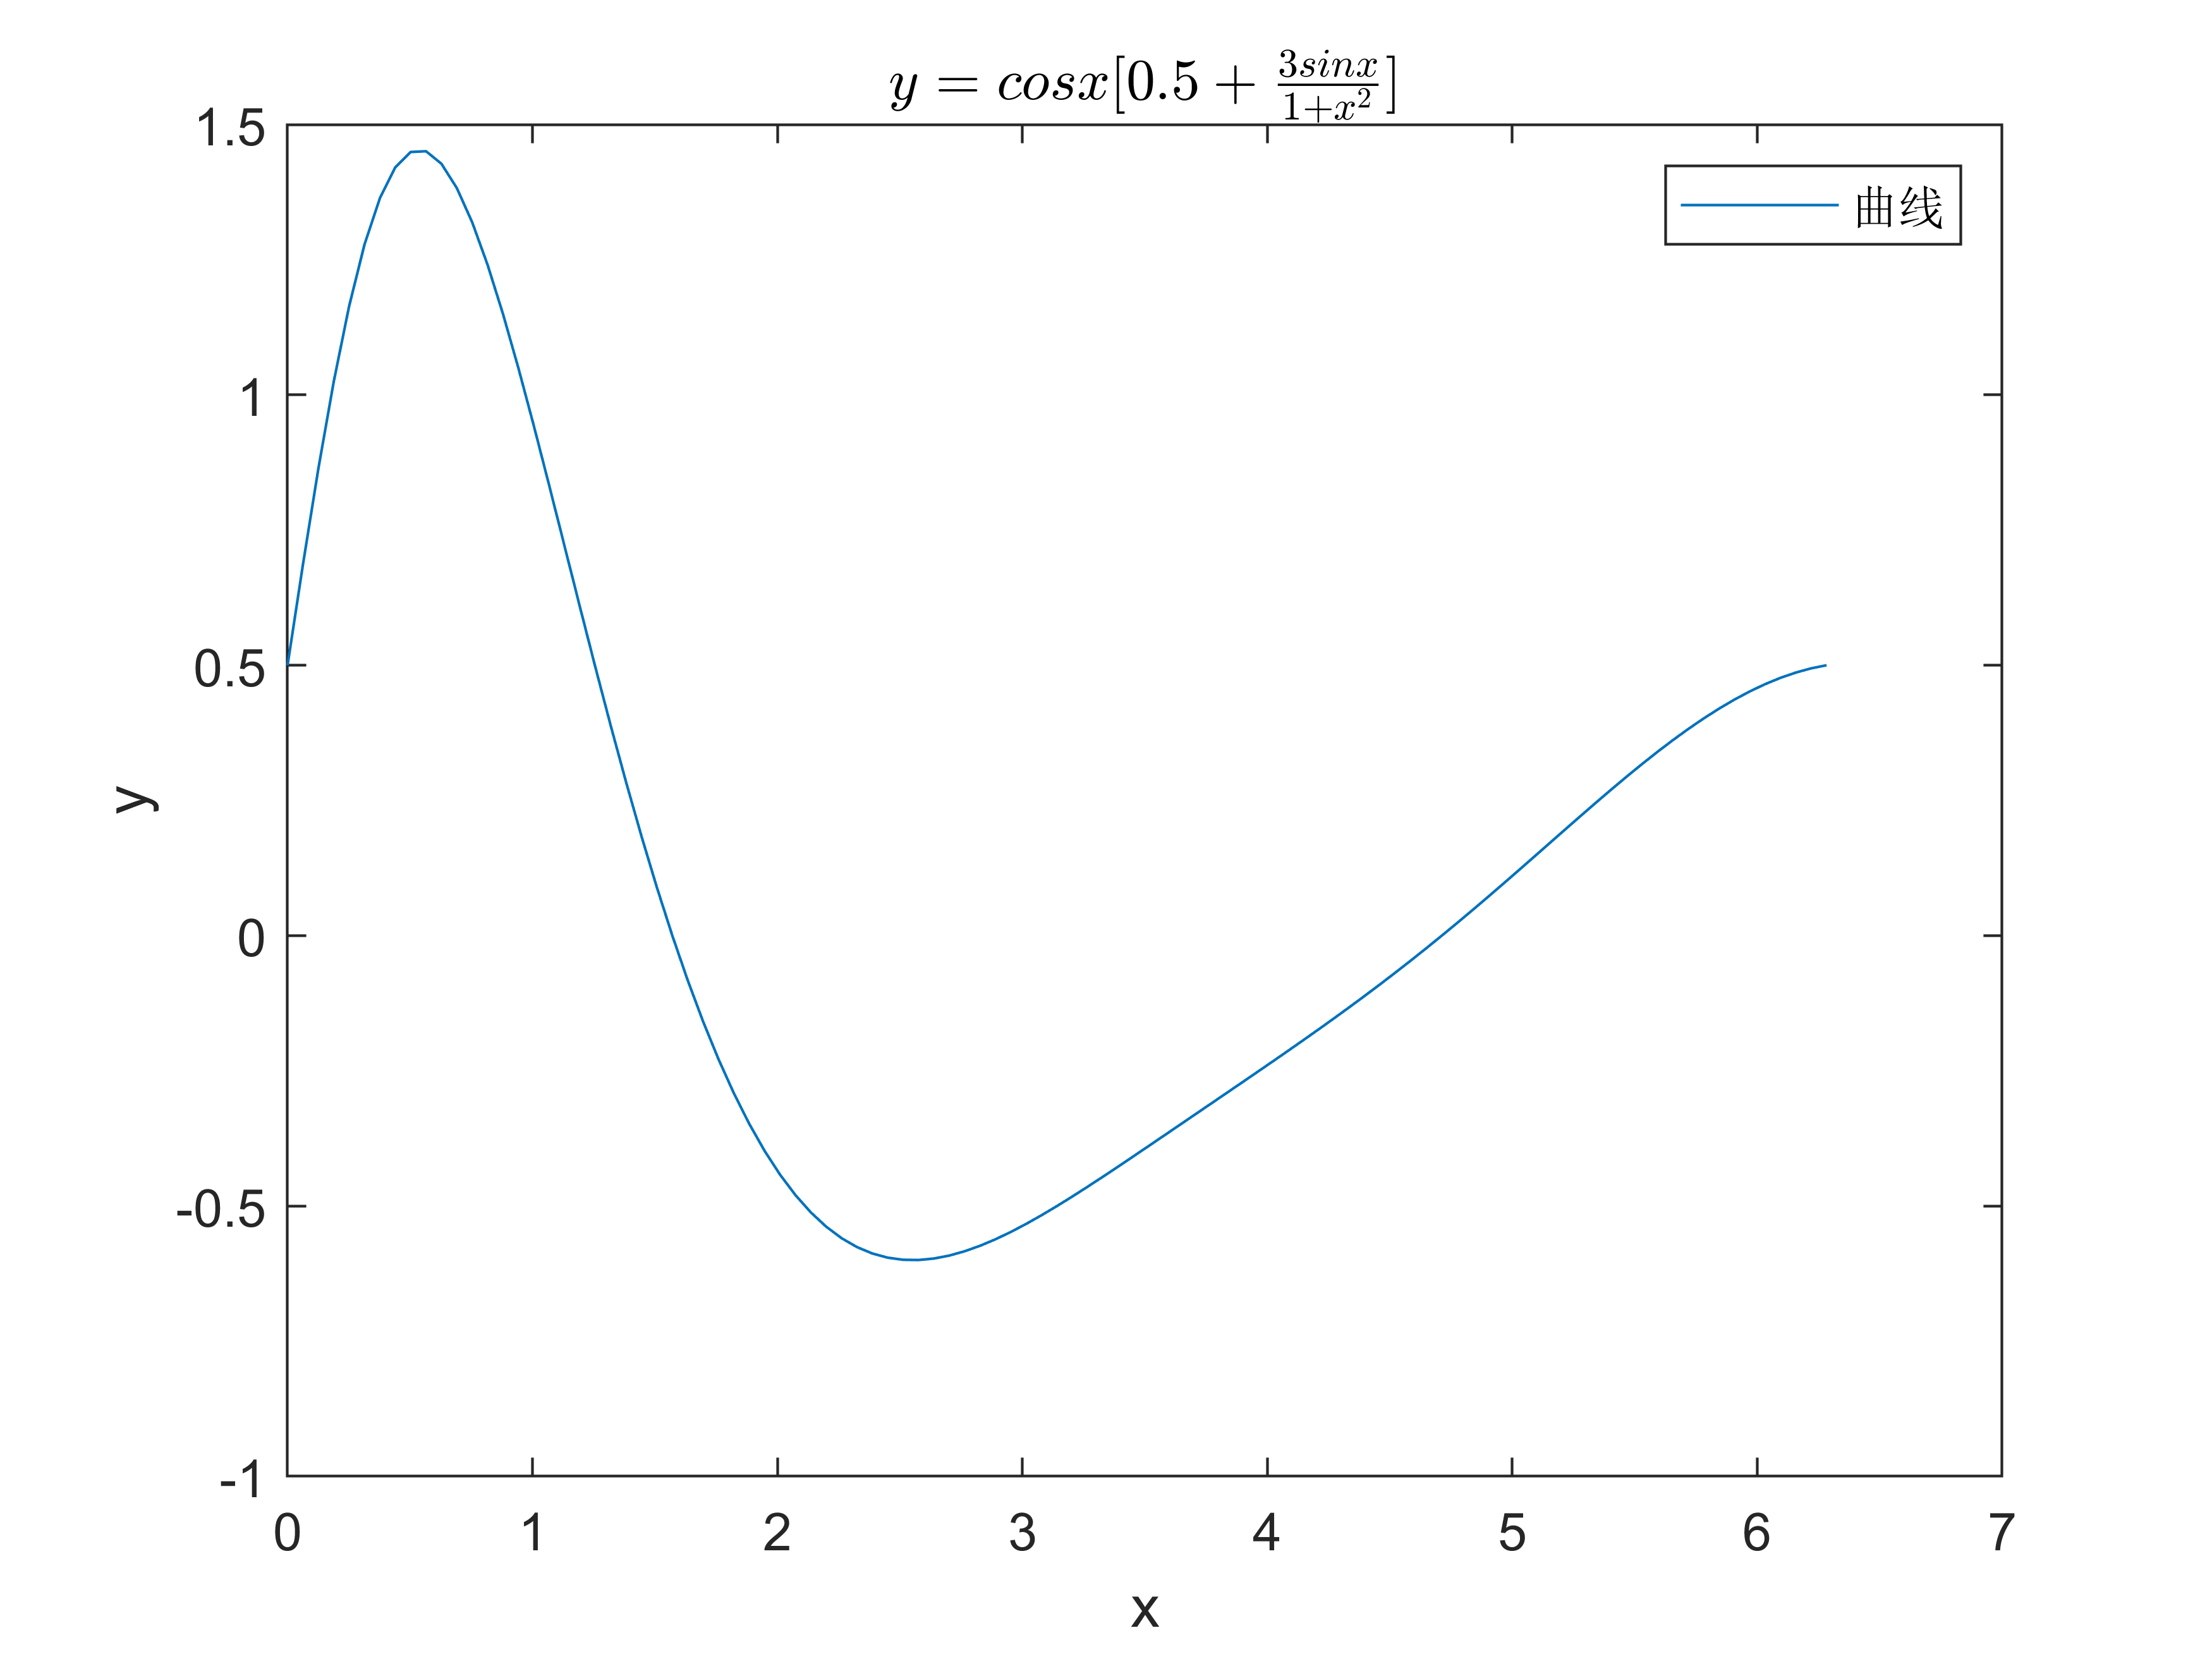
\includegraphics[width=1\textwidth]{T4-1.png}
    \caption{$Plot~y-x$}
    \label{1}
\end{figure}

\section{Signal wave Plot}
\subsection{Description}
Plot $f_1$,$f_2$:
$$
\begin{aligned}
    f_1(t)=&(2-e^(-t)u(t))\\
    f_2(t)=e^(-t)cos&10\pi t[u(t-1)-u(t-2)]\\
    t \in &[0,10]
\end{aligned}
$$

\subsection{Anaylsis}
\noindent Use fucntion plot and stepfun to produce the step vector.\\
Option \textit{title} to produce title name, \textit{xlabel} and \textit{ylabel} to produce 
the text near the Axis.\\
Hold on can let codes plot many times on the figure.\\
\textit{legend} produce the legend of figure to distinguish different curves.
\subsection{Code and Result}
\textbf{Code}
\begin{lstlisting}
clear all;
clc;
t=0:0.01:10;
f1=(2-exp(-t)).*(stepfun(t,0));
f2=exp(-t).*cos(10*pi*t).*(stepfun(t,1)-stepfun(t,2));
plot(t,f1);
hold on;
grid on;
plot(t,f2);
title('Signal waveform');
xlabel('x');
ylabel('y');
legend({'$f_1(t)=(2-e^{-t}u(t)$','$f_2(t)=e^{-t}cos10\pi t[u(t-1)-u(t-2)]$'},'Interpreter','Latex');
\end{lstlisting}
\textbf{Figure}
\begin{figure}[h]
    \centering
    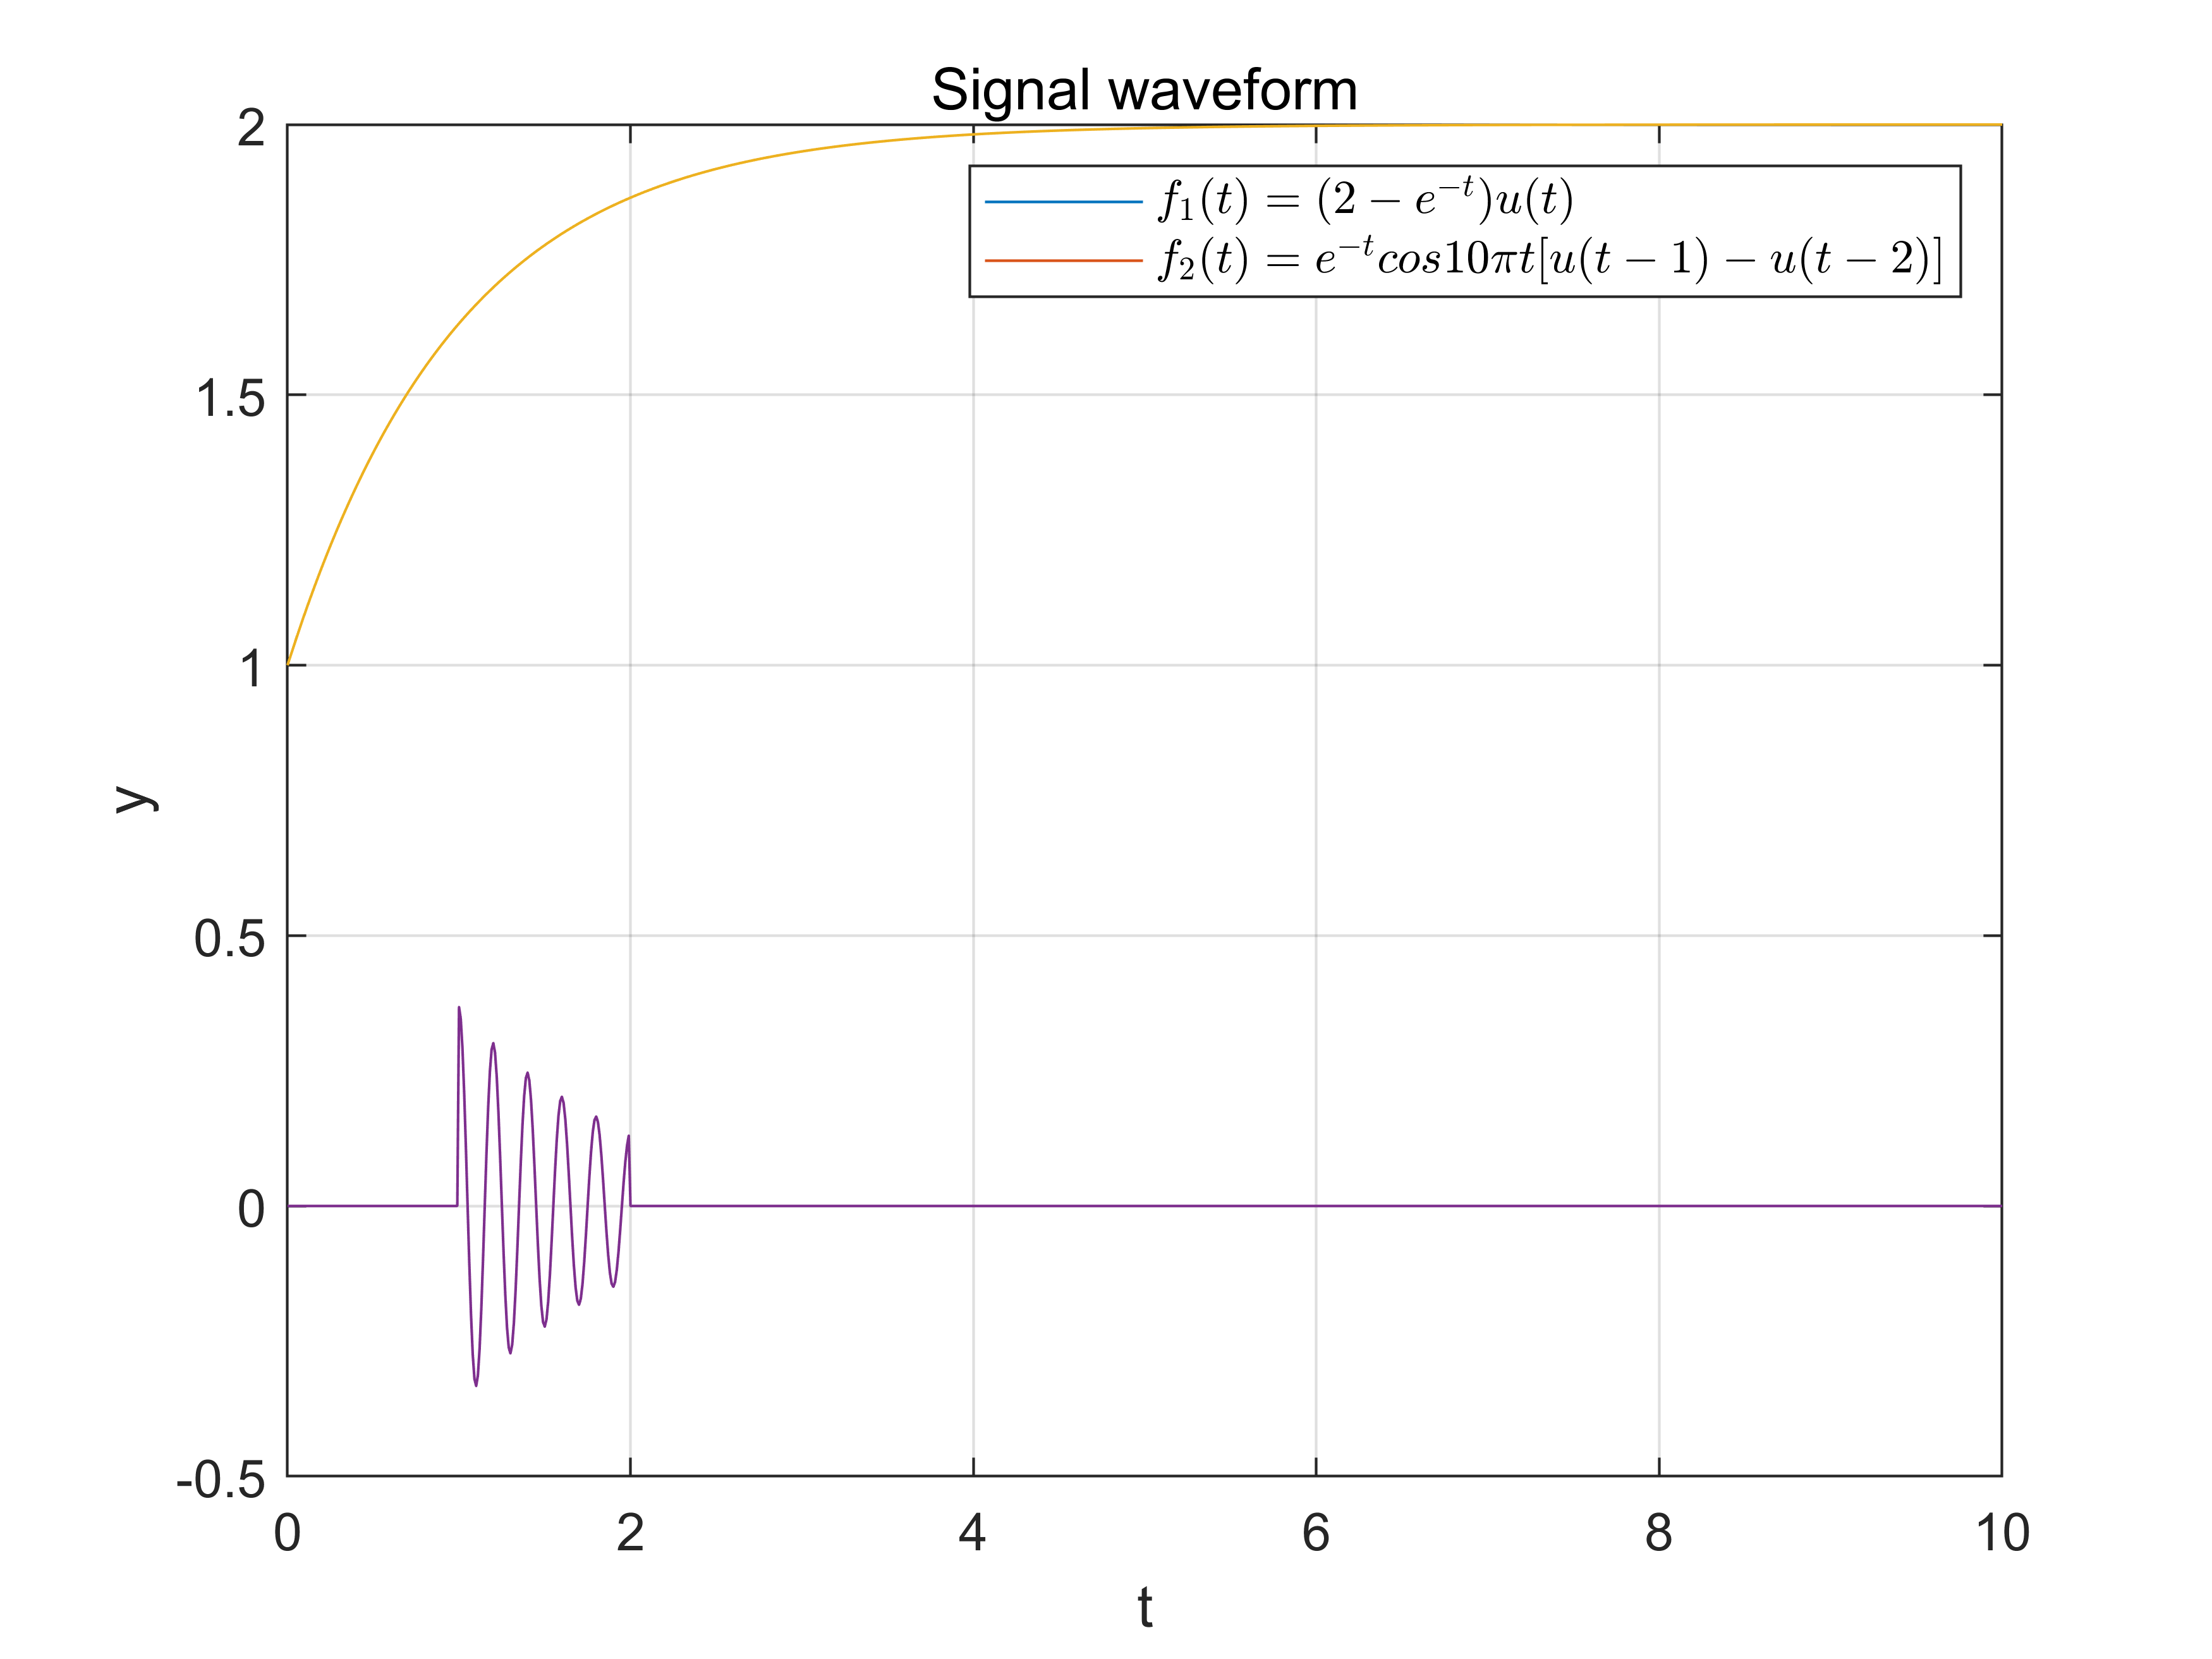
\includegraphics[width=1\textwidth]{T4-2.png}
    \caption{$Plot~Signal~wave$}
    \label{1}
\end{figure}
\section{Parametric Plot}
\subsection{Description}
Plot x-y,
$$
\begin{aligned}
    x=r\cdot cost+3t&,y=r\cdot sint+3\\
    t\in [0,10]&,r=2,3,4
\end{aligned}
$$

\subsection{Anaylsis}
\noindent Use t to produce x,y then plot and change option.\\
gird on to set girds appear on the figure.
\subsection{Code and Result}
\textbf{Code}
\begin{lstlisting}
t=0:0.01:10;
for r=2:4
    x=r*cos(t)+3*t;
    y=r*sin(t)+3;
    plot(y,x);
    hold on;
end
grid on;
title('$x(y),t \in [0,10]$','Interpreter','Latex');
legend('r=2','r=3','r=4');
ylabel({'$x=r\cdot cost+3\cdot t$'},'Interpreter','Latex');
xlabel({'$y=r\cdot cost+3$'},'Interpreter','Latex');
\end{lstlisting}
\newpage
\textbf{Figure}
\begin{figure}[h]
    \centering
    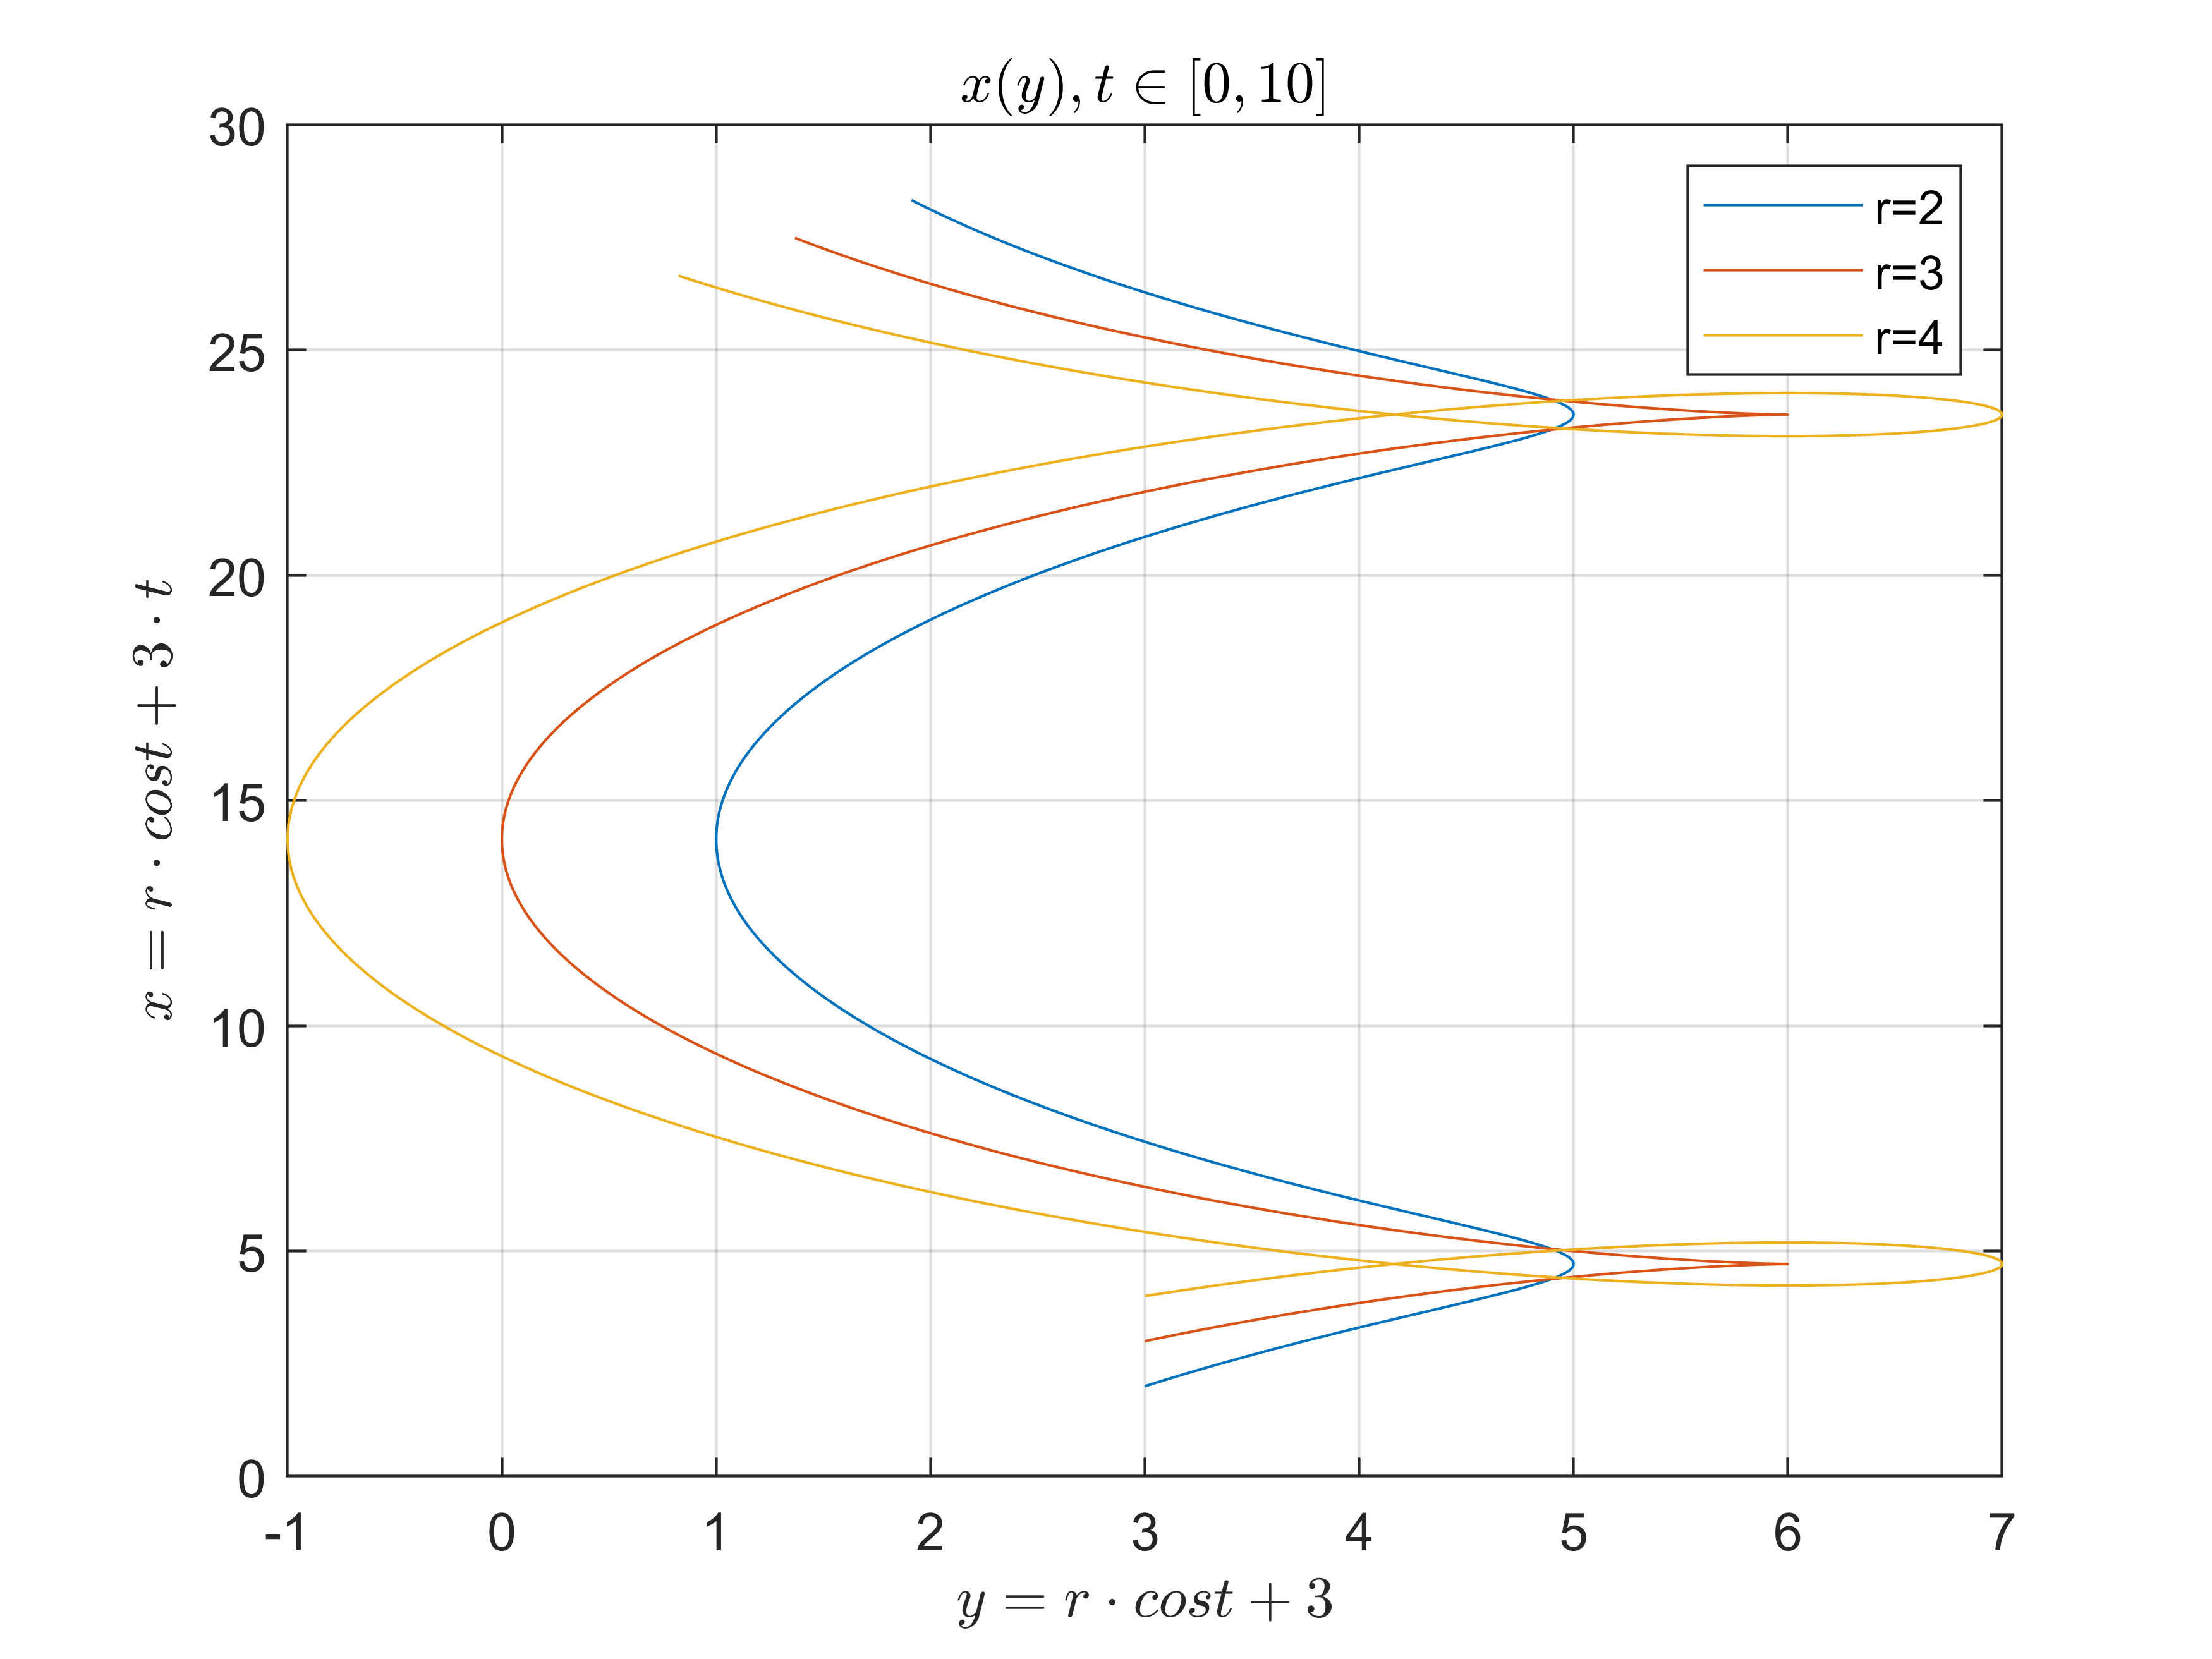
\includegraphics[width=1\textwidth]{T4-3.png}
    \caption{$Parametric~Plot$}
    \label{3}
\end{figure}
\section{Plot option exercise}
\subsection{Description}
\noindent Plot \\
$y_1=1-sin^2(x)$,$y_2=2x+1$,$t \in [0,10]$ on the same figure.\\
requirement:\\
1.$y_1$ is figured by blue circle dots,$y_2$ is figured by green dotted line.\\
2.use legend.\\
3.Axis notes.\\
4.use \textit{gtext} to put \textbf{string 'x=5'} onto the position by click.
\subsection{Anaylsis}
\noindent Give the option different commands according to the requirement.\\
Use \textit{Markersize} and \textit{Linesize} to change the markers and the lines sizes.
\subsection{Code and Result}
\begin{lstlisting}
x=0:0.1:10;
y1=1-sin(x).^2;
y2=2*x+1;
hold on;
grid on;
plot(x,y1,'bO','Markersize',3);
plot(x,y2,'g--');
title('$y1-x,y2-x,x\in [0,10]$','Interpreter','Latex');
legend({'$y1=1-sin^2(x)$','$y2=2x+1$'},'Interpreter','Latex');
axis([0 10 -3 25]);
xlabel('x axis');
ylabel('y axis');
gtext('x=5');
\end{lstlisting}
\textbf{Figure}
\begin{figure}[h]
    \centering
    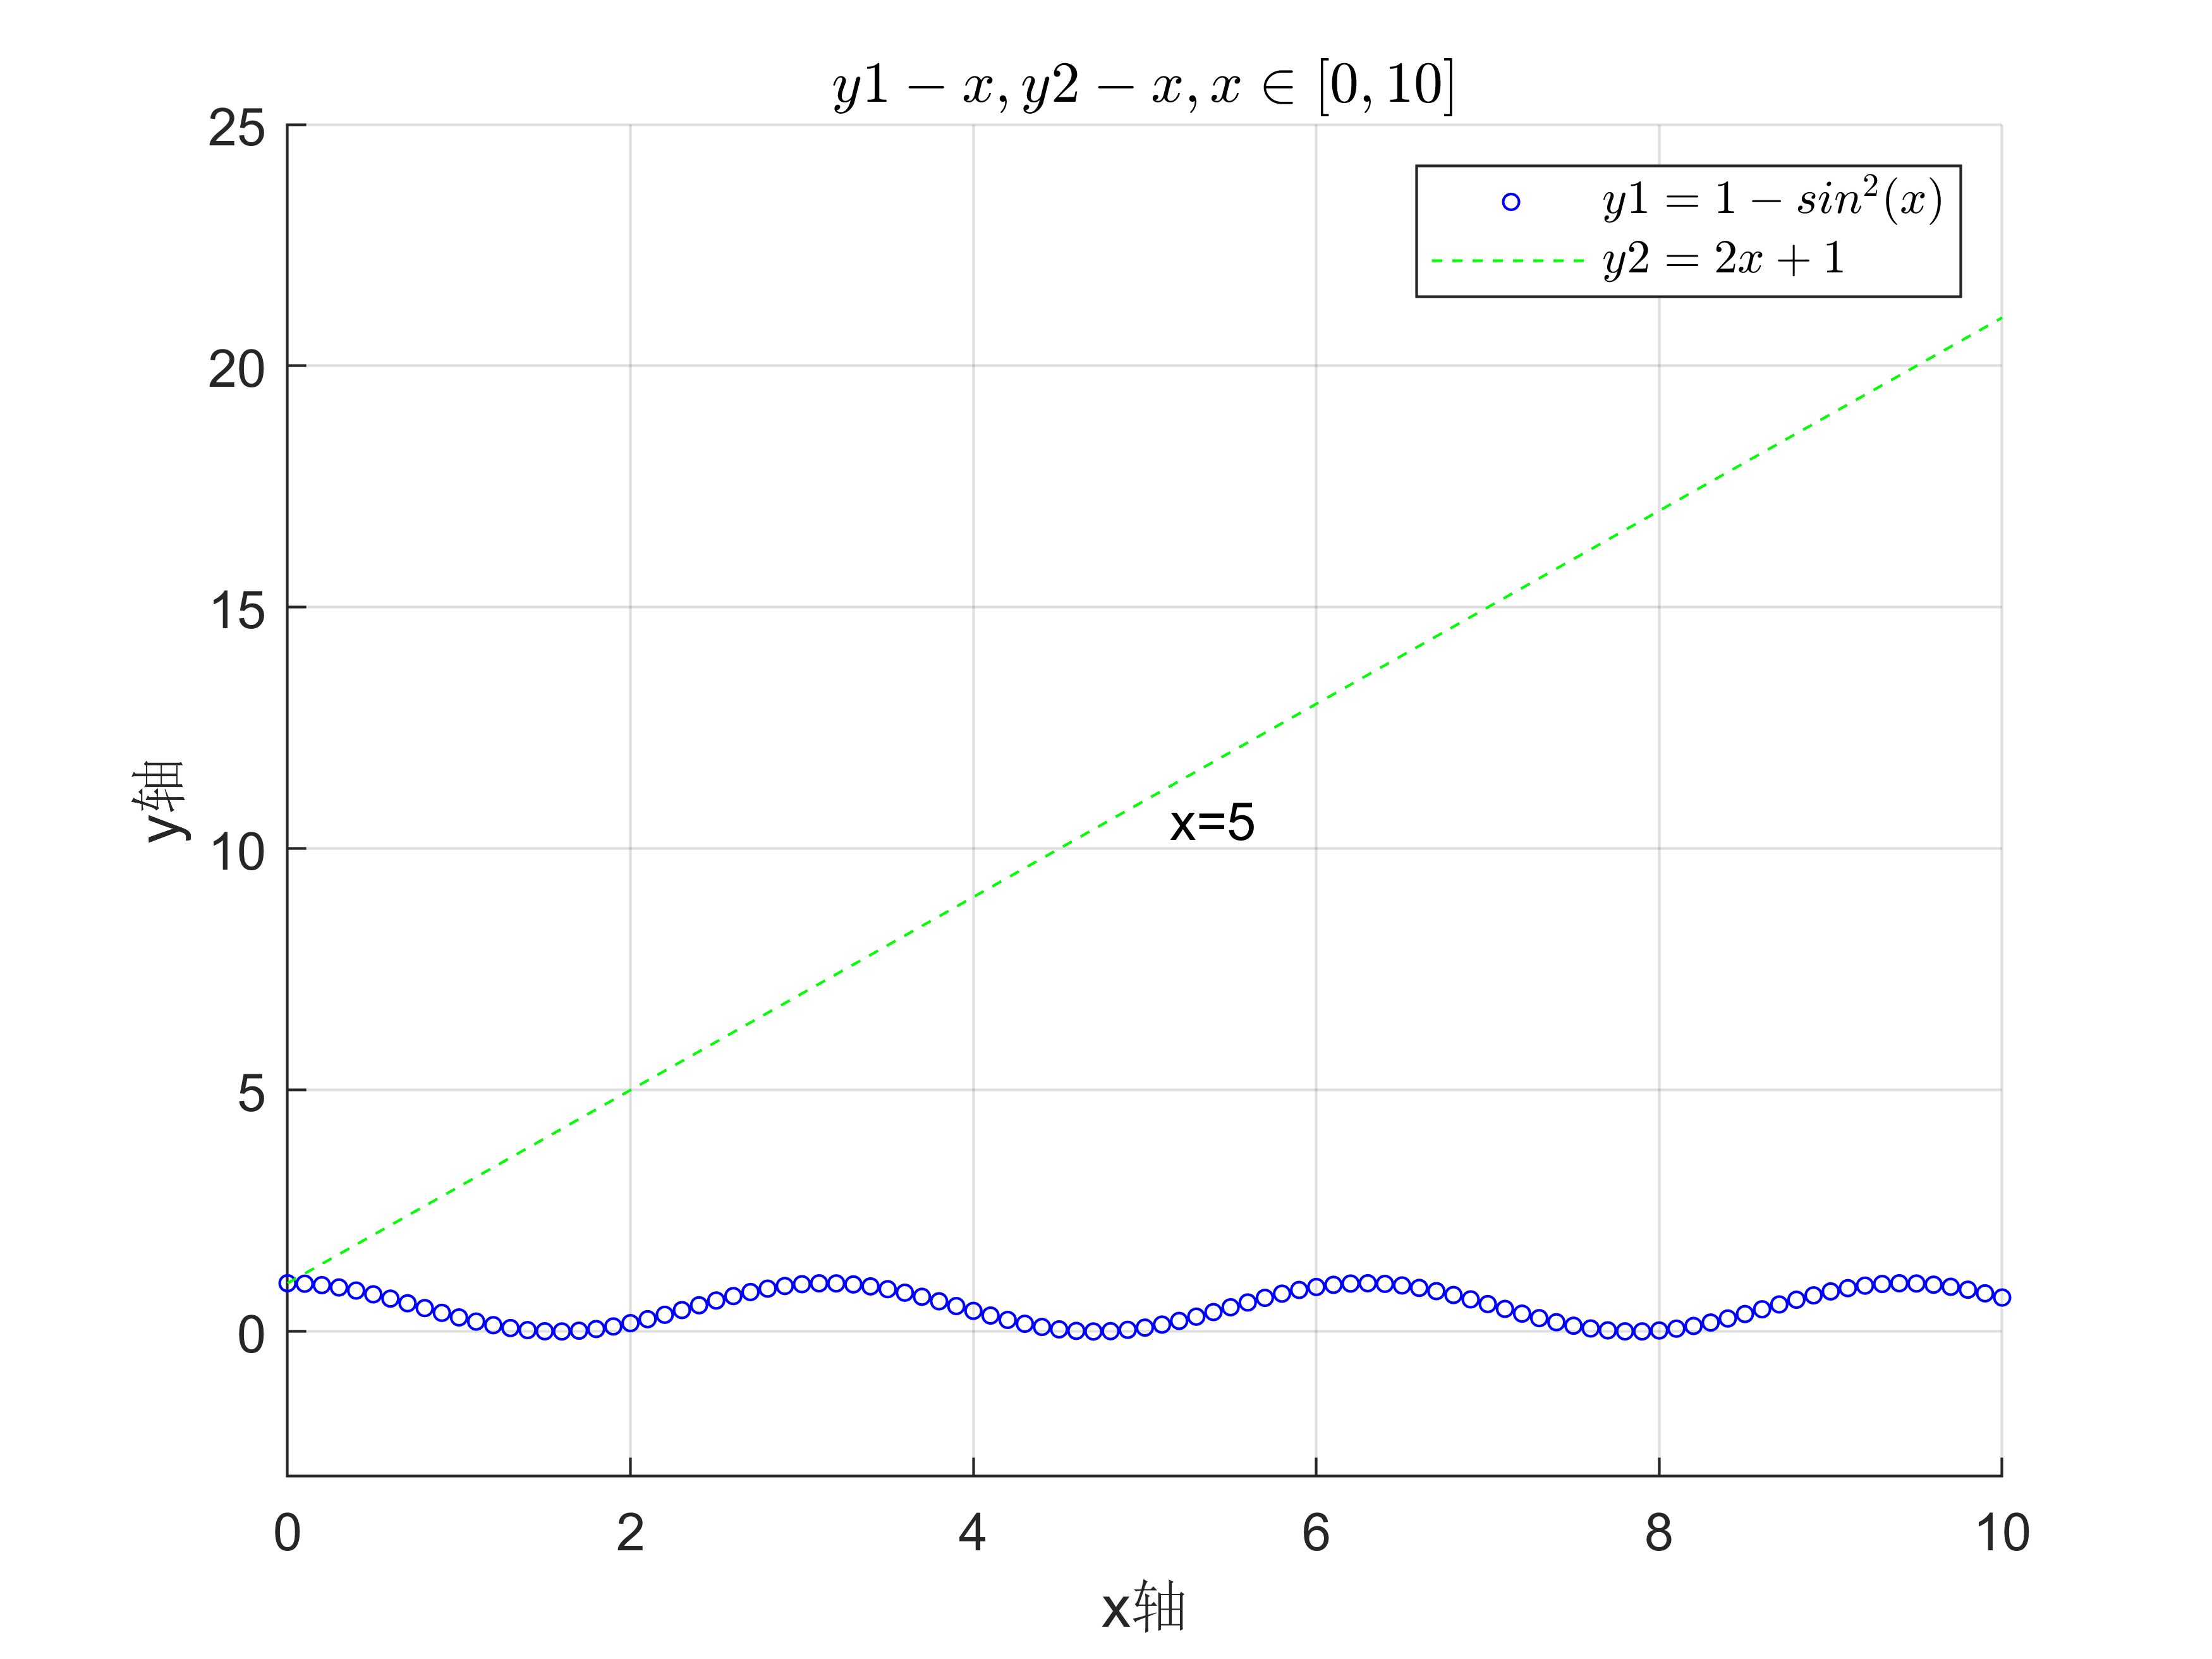
\includegraphics[width=1\textwidth]{T4-4.png}
    \caption{$Options~Plot$}
    \label{4}
\end{figure}
\end{document}